\chapter{Estudo de Análise de Variabilidades de Aplicações Android}

Este capítulo apresenta  o estudo realizado para análise das variabilidades de
aplicações Android. Foram analisados os códigos-fonte de 8 aplicações \textit{open-source},
com o objetivo de identificar e caracterizar as técnicas de implementação de
variabilidades utilizadas em tais aplicações.

O restante desse capítulo está organizado da seguinte maneira: a seção \ref{sec:aplicacoes}
apresenta as aplicações alvo do estudo;  a seção \ref{sec:procedimentos} descreve
os procedimentos adotados na análise; a seção \ref{sec:resultados} mostra os resultados alcançados. 


\section{Aplicações Alvo do Estudo}
\label{sec:aplicacoes}

Nessa fase preliminar, selecionamos um total de 8 aplicações \textit{open-source}
e populares, cada uma com pelo menos 10 mil downloads. Dentro desses critérios,
sete aplicações foram escolhidas de forma aleatória e então foi incluída a
Google I/O\footnote{Aplicação oficial do evento Google I/O. Repositório: https://github.com/google/iosched},
por ser uma aplicação de referência da Google. As demais são aplicações de tamanhos
e categorias variados, possuindo um grande número de usuários. São elas:
Telegram\footnote{Uma aplicação de mensagem. Repositório: https://github.com/DrKLO/Telegram},
AntennaPod\footnote{Um gestor de podcast. Repositório: https://github.com/danieloeh/AntennaPod},
Firefox\footnote{Um navegador web. Repositório: http://hg.mozilla.org/mozilla-central},
Ankidroid\footnote{Um software educativo. Repositório: https://github.com:ankidroid/Anki-Android},
K-9 Mail\footnote{Um cliente de email. Repositório: https://github.com:k9mail/k-9},
C:Geo\footnote{Uma aplicação de geocaching. Repositório: https://github.com:cgeo/cgeo}
e Zmanim\footnote{Um relógio utilizado pelos judeus. Repositório: https://bitbucket.org/jgindin/zmanim}. 

A tabela \ref{tab:aplicacoes}
apresenta maiores informações sobre tais aplicações.
A coluna ID será utilizada para identificar a aplicação em outras tabelas, se necessário.

% Please add the following required packages to your document preamble:
% \usepackage[table,xcdraw]{xcolor}
% If you use beamer only pass "xcolor=table" option, i.e. \documentclass[xcolor=table]{beamer}
\begin{table}[ht]
\centering
\caption{Aplicações analisadas no estudo}
\label{tab:aplicacoes}
\begin{tabular}{|
>{\columncolor[HTML]{FFFFFF}}l |
>{\columncolor[HTML]{FFFFFF}}l |
>{\columncolor[HTML]{FFFFFF}}l |
>{\columncolor[HTML]{FFFFFF}}l |
>{\columncolor[HTML]{FFFFFF}}l |
>{\columncolor[HTML]{FFFFFF}}l |
>{\columncolor[HTML]{FFFFFF}}l |
>{\columncolor[HTML]{FFFFFF}}l |
>{\columncolor[HTML]{FFFFFF}}l |
>{\columncolor[HTML]{FFFFFF}}l |
>{\columncolor[HTML]{FFFFFF}}l |
>{\columncolor[HTML]{FFFFFF}}l |
>{\columncolor[HTML]{FFFFFF}}l |
>{\columncolor[HTML]{FFFFFF}}l |
>{\columncolor[HTML]{FFFFFF}}l |
>{\columncolor[HTML]{FFFFFF}}l |
>{\columncolor[HTML]{FFFFFF}}l |
>{\columncolor[HTML]{FFFFFF}}l |
>{\columncolor[HTML]{FFFFFF}}l |}
\hline
\textbf{ID} & \multicolumn{4}{c|}{\cellcolor[HTML]{FFFFFF}\textbf{Aplicação}} & \multicolumn{4}{c|}{\cellcolor[HTML]{FFFFFF}\textbf{Categoria}}   & \multicolumn{4}{c|}{\cellcolor[HTML]{FFFFFF}\textbf{Downloads}}                                                   & \multicolumn{4}{c|}{\cellcolor[HTML]{FFFFFF}\textbf{\begin{tabular}[c]{@{}c@{}}Nº de linhas\\ de código\end{tabular}}} & \multicolumn{1}{c|}{\cellcolor[HTML]{FFFFFF}\textbf{\begin{tabular}[c]{@{}c@{}}API\\ Mínima\end{tabular}}} & \textbf{\begin{tabular}[c]{@{}l@{}}API\\ Alvo\end{tabular}} \\ \hline
\#1         & \multicolumn{4}{l|}{\cellcolor[HTML]{FFFFFF}Telegram}           & \multicolumn{4}{l|}{\cellcolor[HTML]{FFFFFF}Comunicação}          & \multicolumn{4}{l|}{\cellcolor[HTML]{FFFFFF}\begin{tabular}[c]{@{}l@{}}100.000.000 - \\ 500.000.000\end{tabular}} & \multicolumn{4}{l|}{\cellcolor[HTML]{FFFFFF}576 mil}                                                                   & 9                                                                                                          & 23                                                          \\ \hline
\#2         & \multicolumn{4}{l|}{\cellcolor[HTML]{FFFFFF}AntennaPod}         & \multicolumn{4}{l|}{\cellcolor[HTML]{FFFFFF}Mídia e Vídeo}        & \multicolumn{4}{l|}{\cellcolor[HTML]{FFFFFF}\begin{tabular}[c]{@{}l@{}}100.000 -\\ 500.000\end{tabular}}          & \multicolumn{4}{l|}{\cellcolor[HTML]{FFFFFF}72 mil}                                                                    & 10                                                                                                         & 23                                                          \\ \hline
\#3         & \multicolumn{4}{l|}{\cellcolor[HTML]{FFFFFF}Google I/O}         & \multicolumn{4}{l|}{\cellcolor[HTML]{FFFFFF}Livros e Referências} & \multicolumn{4}{l|}{\cellcolor[HTML]{FFFFFF}\begin{tabular}[c]{@{}l@{}}500.000 -\\ 1.000.000\end{tabular}}        & \multicolumn{4}{l|}{\cellcolor[HTML]{FFFFFF}66 mil}                                                                    & 14                                                                                                         & 22                                                          \\ \hline
\#4         & \multicolumn{4}{l|}{\cellcolor[HTML]{FFFFFF}Firefox}            & \multicolumn{4}{l|}{\cellcolor[HTML]{FFFFFF}Comunicação}          & \multicolumn{4}{l|}{\cellcolor[HTML]{FFFFFF}\begin{tabular}[c]{@{}l@{}}100.000.000 -\\ 500.000.000\end{tabular}}  & \multicolumn{4}{l|}{\cellcolor[HTML]{FFFFFF}279 mil}                                                                   & 15                                                                                                         & 22                                                          \\ \hline
\#5         & \multicolumn{4}{l|}{\cellcolor[HTML]{FFFFFF}AnkiDroid}          & \multicolumn{4}{l|}{\cellcolor[HTML]{FFFFFF}Educação}             & \multicolumn{4}{l|}{\cellcolor[HTML]{FFFFFF}\begin{tabular}[c]{@{}l@{}}1.000.000 - \\ 5.000.000\end{tabular}}     & \multicolumn{4}{l|}{\cellcolor[HTML]{FFFFFF}93 mil}                                                                    & 10                                                                                                         & 22                                                          \\ \hline
\#6         & \multicolumn{4}{l|}{\cellcolor[HTML]{FFFFFF}K-9 Mail}           & \multicolumn{4}{l|}{\cellcolor[HTML]{FFFFFF}Comunicação}          & \multicolumn{4}{l|}{\cellcolor[HTML]{FFFFFF}\begin{tabular}[c]{@{}l@{}}5.000.000 -\\ 10.000.000\end{tabular}}     & \multicolumn{4}{l|}{\cellcolor[HTML]{FFFFFF}123 mil}                                                                   & 15                                                                                                         & 22                                                          \\ \hline
\#7         & \multicolumn{4}{l|}{\cellcolor[HTML]{FFFFFF}C:Geo}              & \multicolumn{4}{l|}{\cellcolor[HTML]{FFFFFF}Entretenimento}       & \multicolumn{4}{l|}{\cellcolor[HTML]{FFFFFF}\begin{tabular}[c]{@{}l@{}}1.000.000 - \\ 5.000.000\end{tabular}}     & \multicolumn{4}{l|}{\cellcolor[HTML]{FFFFFF}149 mil}                                                                   & 9                                                                                                          & 21                                                          \\ \hline
\#8         & \multicolumn{4}{l|}{\cellcolor[HTML]{FFFFFF}Zmanim}             & \multicolumn{4}{l|}{\cellcolor[HTML]{FFFFFF}Estilo de Vida}       & \multicolumn{4}{l|}{\cellcolor[HTML]{FFFFFF}\begin{tabular}[c]{@{}l@{}}10.000 -\\ 50.000\end{tabular}}            & \multicolumn{4}{l|}{\cellcolor[HTML]{FFFFFF}48 mil}                                                                    & 10                                                                                                         & 22                                                          \\ \hline
\end{tabular}
\end{table}

Nos arquivos de configuração das aplicações, são definidas as versões mínima e
alvo da API necessária para o execução da aplicação. Se por um lado, os desenvolvedores
desejam utilizar os recursos mais modernos da plataforma, por outro desejam ter
suas aplicações instaladas na maior quantidade possível de dispositivos. Dessa
forma, a aplicação pode estar preparada para funcionar em versões antigas da
API, sem abrir mão de usar os últimas novidades. As versões mínimas encontradas
nas 8 aplicações variaram de 9 (Telegram e C:geo) a 15 (Firefox e K-9 Mail),
enquanto que apenas uma aplicação estava otimizada para a versão 21, duas
aplicações para versão mais recente (23 - Telegram e AntennadPod) e as demais
para versão 22.


\section{Procedimentos}
\label{sec:procedimentos}
Uma vez selecionadas as aplicações alvos do nosso estudo, foi realizada a atividade
de análise das aplicações para entender as soluções adotadas tanto em relação
as versões da API, quanto em relação a diferentes tamanhos de telas.

Para análise do tratamento das diferentes versões da API foram realizados os seguintes passos: 
\begin{enumerate}
    \item Pesquisa textual por \texttt{VERSION.SDK\_INT} em todos os arquivos da
        aplicação.
        Essa constante indica a versão da API do dispositivo e normalmente está
        em uma instrução condicional;
    \item Análise do contexto dos resultados de 1 para determinar se:
        \begin{enumerate}
            \item Trata-se da implementação do padrão Execução Condicional \cite{Santos2012};
            \item Ou a implementação é baseada em padrões de projeto \cite{Gamma1994}. 
        \end{enumerate}
    \item Pesquisa por referencias ao pacote android.support, indicando que a aplicação 
        faz uso do pacote de compatibilidade oficial.
\end{enumerate}

Para uma aplicação prover suporte a dispositivos com diferentes tamanhos de tela,
de acordo com o guia oficial para desenvolvedores \cite{supporting_tablets},
são necessários seguir alguns passos:
\begin{enumerate}
    \item Construir as telas usando a API de fragmentos;
    \item Utilizar \textit{action bar}, um componente visual que substitui a barra
        superior
        das aplicações e, por padrão, inclui o logo no lado esquerdo, seguido pelo
        título da \textit{activity},  e o menu da aplicação no lado direito.
    \item Implementação de layouts flexíveis, que permitirão às aplicações
        adaptarem-se a variações de telas diferentes. Não só em relção a dimensões,
        mas também em relação a densidade - a quantidade de pixels por área física
        da tela.    
\end{enumerate}

Os itens 1 e 2 acima implicam na necessidade da versão 11 da API ou do uso do
pacote de compatibilidade e estensão das classes \texttt{FragmentActivity} para
uso de fragmentos ou \texttt{AppCompatActivity} e uso tema \texttt{Theme.AppCompat}
para \textit{action bar}. Além disso, em tempo de execução a interface do aplicativo
deve ser composta de acordo com o tamanho da tela do dispositivo e fragmentos disponíveis.

Dessa forma, os passos para análise da variabilidade de tratamento de tamanhos
de telas diferentes foram os seguintes: 
\begin{enumerate}
    \item Verificação se a \textit{activity} principal da aplicação estende da
        classe \textit{FragmentActivity}. Se essa estensão é identificada, os
        passos 2 a 4 são realizados, caso contrário pula-se para o passo 5;
    \item Verificação se no método \texttt{onCreate()} da \textit{activity}
        principal ocorre composição de telas com uso de fragmentos;
    \item Verificação se a \textit{activity} principal da aplicação estende as
        classes \texttt{AppCompatActivity} ou \texttt{ActionBarActivity}.
        A segunda classe foi depreciada em favor da primeira, por isso optou-se
        por verificar uma ou outra;
    \item Verificação se a \textit{activity} utiliza o tema \texttt{Theme.AppCompat} ou um compatível;
    \item Verificar na diretório de recursos das aplicação (\texttt{res}) a existência
        de recursos específicos para diferentes telas;
    \item Instalação e da aplicação em dispositivos com tamanhos de telas e versão
        da API diferentes.
\end{enumerate}

\section{Resultados do Estudo}
\label{sec:resultados}

Essa seção apresenta e discute os resultados do estudo. Inicialmente, na seção 
\ref{sec:tecnicas} são discutidos as técnicas de implementação para lidar com
diferentes versçoes da API. A seção \ref{sec:mudancas} discute mudanças na API
com maior impacto no desenvolvimento das aplições.
Na seção \ref{sec:multiplas_telas} são apresentados os
resultados para o tratamento de múltiplas telas. Na seção \ref{sec:multiplos_pacotes}
é discutido o recurso provido pela plataforma de múltiplos pacotes para instalação.
Por fim, a seção \ref{sec:ferramentas} apresenta ferramentas úteis para tratar variabilidades. 

\subsection{Técnicas de Implementação de Variabilidades na API}
\label{sec:tecnicas}

De forma a permitir a implementação das aplicações contemplando as diferentes versões,
diferentes técnicas de implementação foram identificadas para lidar com esse problema.
A Tabela \ref{tab:tecnicas} apresenta essas diferentes alternativas de projeto
encontradas nas aplicações analisadas.

\begin{table}[ht]
\centering
\caption{Técnicas de implementação de variabilidades na API encontrados nas aplicações}
\label{tab:tecnicas}
\resizebox{\textwidth}{!}{
\begin{tabular}{|c|c|l|l|l|c|l|l|l|c|l|l|l|c|l|l|l|c|c|}
\hline
\textbf{\begin{tabular}[c]{@{}c@{}}Pacote de\\ compatibilidade\end{tabular}} & \multicolumn{4}{c|}{\textbf{\begin{tabular}[c]{@{}c@{}}Execução\\ Condicional\end{tabular}}} & \multicolumn{4}{c|}{\textbf{\begin{tabular}[c]{@{}c@{}}Reimplementação\\ de Recursos\end{tabular}}} & \multicolumn{4}{c|}{\textbf{\begin{tabular}[c]{@{}c@{}}PP\\ Proxy\end{tabular}}} & \multicolumn{4}{c|}{\textbf{\begin{tabular}[c]{@{}c@{}}PP\\ Strategy\end{tabular}}} & \textbf{\begin{tabular}[c]{@{}c@{}}PP\\ Null Object\end{tabular}} & \textbf{\begin{tabular}[c]{@{}c@{}}PP\\ Decorator\end{tabular}} \\ \hline
\begin{tabular}[c]{@{}c@{}}Todas as \\ aplicações\end{tabular}               & \multicolumn{4}{c|}{\begin{tabular}[c]{@{}c@{}}Todas as\\ aplicações\end{tabular}}           & \multicolumn{4}{c|}{Telegram}                                                                       & \multicolumn{4}{c|}{\begin{tabular}[c]{@{}c@{}}Telegram\\ c:geo\end{tabular}}    & \multicolumn{4}{c|}{\begin{tabular}[c]{@{}c@{}}AnkiDroid\\ K-9 Mail\end{tabular}}   & c:geo                                                             & c:geo                                                           \\ \hline
\end{tabular}
}
\end{table}

\subsubsection{Pacote de Compatibilidade}
Pacotes de compatibilidade permitem que aplicações em execução sob versão antigas
da plataforma utilizem recursos que foram disponibilizados em versões mais novas.
Por exemplo, uma aplicação instalada em um celular com versão 8 pode usar a API
de fragmentos, disponibilizada apenas na versão 11.

Esses pacotes são tradicionais arquivos JAR com classes, interfaces e outros
artefatos de recursos que poderão ser adicionados na aplicação. Assim, quando se
deseja usar a classe \texttt{Fragment}, por exemplo, em vez da importação ser da API padrão
do Android, como mostra a Figura \ref{fig:import_fragment_API}, deverá ser desse pacote que
está junto da aplicação, como mostrado na Figura \ref{fig:import_fragment_compat}.

\begin{figure}[ht]
\centering
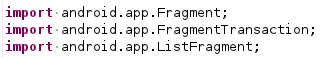
\includegraphics{imagens/import_fragment_api.png}
\caption{ Importando classes relacionadas a fragmentos da API padrão}
\label{fig:import_fragment_API}
\end{figure}

\begin{figure}[ht]
\centering
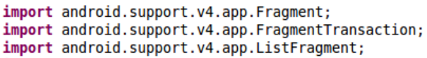
\includegraphics{imagens/import_fragment_compat.png}
\caption{Importando classes relacionadas a fragmentos do pacote de compatibilidde}
\label{fig:import_fragment_compat}
\end{figure}

Como resultado, a aplicação será distribuída com uma experiência de uso mais
consistente através de uma grande número de versões da plataforma.

Uso do pacote de compatibilidade oficial foi a forma mais comum para prover
suporte aos dispositivos com versões antigas, sendo utilizada por todos os
aplicativos analisados.

A tabela \ref{tab:criterios_pacote} descreve o pacote de compatibilidade
segundo o framework de comparação apresentado na seção \ref{sec:framework}

\begin{table}[ht]
\centering
\caption{Descrição do pacote de compatibilidade segundo o framework de comparação}
\label{tab:criterios_pacote}
\begin{tabular}{|l|l|}
\hline
\multicolumn{1}{|c|}{\textbf{Critério de Avaliação}}                                                    & \multicolumn{1}{c|}{\textbf{Valor obtido}} \\ \hline
Tipo de Variabilidade                                                                                   & Ambos                                      \\ \hline
Variabilidade na estrutura                                                                              & Oferece suporte                            \\ \hline
Variabilidade no comportamento                                                                          & Oferece suporte                            \\ \hline
Granularidade                                                                                           & Grossa                                     \\ \hline
Tempo de ligação                                                                                        & Compilação                                 \\ \hline
Reusabilidade                                                                                           & Alta                                       \\ \hline
Legibilidade                                                                                            & Baixo impacto                              \\ \hline
Desempenho                                                                                              & Baixo impacto                              \\ \hline
Tamanho da aplicação                                                                                    & Médio impacto                              \\ \hline
\begin{tabular}[c]{@{}l@{}}Suporte para implementação\\ modular de requisitos transversais\end{tabular} & Não oferece suporte                        \\ \hline
\end{tabular}
\end{table}

Pacotes de compatibilidade substituem de forma estática componentes de versões anteriores
da API por componentes de novas versões, de forma que oferece suporte para o tipo
de variabilidades positivas e negativas. Também oferece suporte à granularidade grossa,
já que os componentes são substuídos por completo. Tal substituição equivale tanto
a adicionar
quanto a remover métodos e atributos nas classes, ou sobrescrever os existentes,
portanto essa técnica oferece suporte para variabilidade na estrutura e no comportamento.
Essa técnica também exerce um baixo impacto na legibilidade do código e no desempenho da aplicação. 
Uma vez que, na maioria dos casos, basta alterar a importação das classes, como
mostramos nas figuras \ref{fig:import_fragment_API} e \ref{fig:import_fragment_compat}.
No entanto, pode resultar em um aumento no tamanho da aplicação, ou no caso particular
do Android, um estouro no limite de métodos das aplicações \cite{multidex},
já que o tempo de ligação dessa técnica é durante a compilação e mais elementos
serão empacotados juntamente com a aplicação. Não oferece suporte para implementação
modular de requisitos transversais.

\subsubsection{Execução Condicional}
Execução condicional (EC) é um padrão para tratar variabilidades em granularidade
fina em linhas de produto de software \cite{Santos2012}. O padrão é composto
por 4 elementos principais, ilustrados na Figura \ref{fig:EC}:
\begin{itemize}
    \item Classe alvo: componentes do sistema onde ocorre a variabilidade acontece; 
    \item Implementação da variabilidade: o código que representa a variabilidade,
        podendo ser um trecho diretamente na classe algo ou uma chamada para um
        componente que implementa a variabilidade; 
    \item Gerenciador da execução: é um elemento central do padrão, responsável
        por decidir qual implementação da variabilidade será executada. 
    \item Repositório de parâmetros:  responsável por armazenar os valores dos
        parâmetros que será utilizado durante a execução condicional. É fundamental
        que a recuperação desses parâmetros não prejudique o desempenho das aplicações.
\end{itemize}

\begin{figure}[ht]
\centering
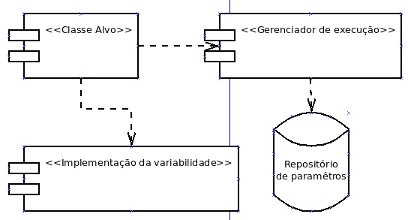
\includegraphics{imagens/execucao_condicional.png}
\caption{Componentes principais do padrão execução condicional}
\label{fig:EC}
\end{figure}

Em aplicações Android, as classes alvo podem ser qualquer classe da aplicação.
Gerenciador de execução é uma instrução \texttt{if} que compara a versão da API
no dispositivo à uma versão cujo valor tem alguma importância para a variabilidade
em questão. Por exemplo, a versão em que um recurso surgiu ou mudou de comportamento.
Implementação da variabilidade costuma ser uma sequência de código para quando o
resultado dessa comparação é verdadeiro e outra sequência para quando ele é falso.
O repositório de parâmetros que armazenar os valores utilizados nesse contexto é a
classe \texttt{android.os.Build}, que contém diversas sobre o sistema instalado
no aparelho, e suas classes aninhadas \texttt{VERSION} e \texttt{VERSION\_CODES}.
Em particular, a versão da API é obtida no atributo \texttt{Build.VERSION\_CODES.SDK\_INT},
já o outro valor da comparação é normalmente definida diretamente no código ou obtido de
\texttt{VERSION\_CODES}.  

A figura \ref{fig:exemploEC} apresenta um exemplo do uso de EC na aplicação c:geo. 
Nesse exemplo, a classe alvo definida no padrão é a classe \texttt{AbstractDialogFragment}
, do repositório
de parâmetros são obtidos os valores de \texttt{Build.VERSION.SDK\_INT} e
\texttt{Build.VERSION\_CODES.HONEYCOMB}, para serem utilizados na condição do \texttt{if...else}, 
que faz o papel de gerenciador de execução. Também vemos que existem duas
implementação de variabilidade: i) uma composta apenas por uma linha de código
(\texttt{view.showContextMenu()}); e ii) a outra composta por várias linhas e
encapsulada no método \texttt{showPopupHoneycomb(View view)}.

\begin{figure}[ht]
\centering
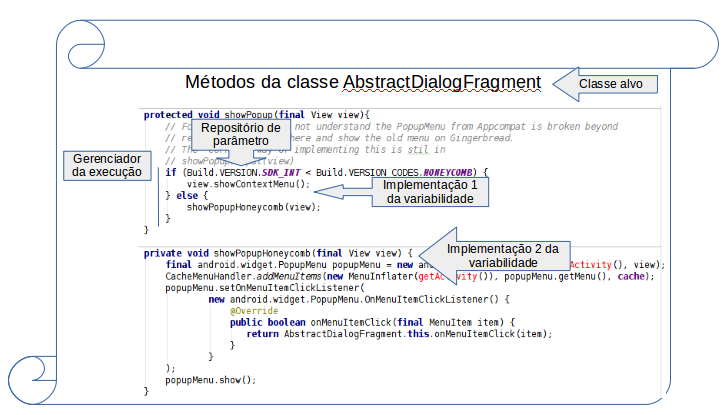
\includegraphics[width=1\textwidth]{imagens/EC_in_cgeo2.png}
\caption{Exemplo do padrão EC no cgeo}
\label{fig:exemploEC}
\end{figure}

Assim como uso do pacote de compatibilidade, EC foi observado em todas as aplicações.
A tabela \ref{tab:criterios_EC} descreve essa técnica
segundo o framework de comparação apresentado na seção \ref{sec:framework}

\begin{table}[ht]
\centering
\caption{Descrição do padrão execução condicional segundo o framework de comparação}
\label{tab:criterios_EC}
\begin{tabular}{|l|l|}
\hline
\multicolumn{1}{|c|}{\textbf{Critério de Avaliação}}                                                    & \multicolumn{1}{c|}{\textbf{Valor obtido}} \\ \hline
Tipo de Variabilidade                                                                                   & Ambos                                      \\ \hline
Variabilidade na estrutura                                                                              & Não oferece suporte                        \\ \hline
Variabilidade no comportamento                                                                          & Oferece suporte                            \\ \hline
Granularidade                                                                                           & Fina, grossa                               \\ \hline
Tempo de ligação                                                                                        & Execução                                   \\ \hline
Reusabilidade                                                                                           & Baixa                                      \\ \hline
Legibilidade                                                                                            & Médio impacto                              \\ \hline
Desempenho                                                                                              & Baixo impacto                              \\ \hline
Tamanho da aplicação                                                                                    & Baixo impacto                              \\ \hline
\begin{tabular}[c]{@{}l@{}}Suporte para implementação\\ modular de requisitos transversais\end{tabular} & Não oferece suporte                        \\ \hline
\end{tabular}
\end{table}

EC oferece suporte para ambos os tipos de variabilidade, positiva e negativa,
dado que o gerenciador de execução pode executar algo a mais do núcleo da aplicação
(positiva) ou deixar de executar algo desse núcleo (negativa).

Uma vez que o tempo de ligação é durante a  execução, essa técnica não oferece
suporte para variabilidade na estrutura, apenas no comportamento. No entanto,
isso pode ser alcançado combinado com o uso de pacote de compatibilidade pela
implementação de variabilidades. E, apesar do tempo de ligação ser na execução,
o que pode implicar em repetidos desvios condicionais, a impacto no desempenho é
baixo, graças ao mecanismo do repositório de parâmentros, que apenas obtém o valor
de um atributo estático de uma classe.

EC pode definir o tipo dos objetos a serem criados, oferecendo suporte à granularidade
grossa, ou apenas a execução ou não de uma linha de código qualque, suporte à
granularidade fina. No último caso, que é mais comum,  reusabilidade e
legibilidade são prejudicadas.

Para verificar o impacto no tamanho da aplicação, realizamos uma grande refatoração
em uma das aplicações, o Telegram. Eliminamos todas as EC condicionadas a versão da
API, deixando o mesmo com suporte apenas para versão 23 da plataforma. Um total
de 145 arquivos foram editados ou apagados. Comparando os tamanhos dos arquivos
APK (Android Package) dessa versão e da versão com suporte a partir da API 9 não foi verificada
diferença alguma. Portanto, essa técnica tem baixo impacto no tamanho das aplicações.

EC não oferece suporte para implementação modular de requisitos transversais.

Apesar de execução condicional trazer uma baixa legibilidade no código, seu uso
é bastante simples e comum, não exigindo conhecimentos avançados e nem uso de
ferramentas externas, como exige a técnica de compilação condicional (CC) \cite{Medeiros2015}.
A técnica de CC é bastante utilizada em outras plataformas para gerencia de
variabilidades \cite{Liebig2010}, entretanto não foi observado seu uso em
nenhuma das aplicações analisadas no nosso estudo. Dois fatores podem contribuir
para a baixa legibilidade: (i) o código de todas as variabilidades estarão presentes
em todos produtos da LPS; (ii) uso de \texttt{Build.VERSION\_CODES}. O primeiro é 
intriseco ao padrão, já o segundo é específico da plataforma Android. A classe
\texttt{Build.VERSION\_CODES} contém atributos que mapeiam a versão da API. Quando
eles são utilizados no código, frequentemente é necessário recorrer à tabela presente
na figura \ref{fig:platform_versions}.

\subsubsection{Reimplementação de recursos}
\label{sec:reimplementacao}
Reimplementação de recursos ocorre quando se deseja um comportamento já provido
por versões mais recentes ou outra biblioteca, mas opta-se por reimplementar tal
recurso. Foi verificado que apenas o Telegram optou por essa abordagem, quando
reimplementou algumas classes relacionadas a animações gráficas, quando poderia
ter utilizado um pacote de compatibilidade  com o recurso pronto. A figura \ref{fig:telegram_diretorio}
apresente a estrutura de pacotes do Telegram, com destaque para as classes que 
reimplementam o pacote \texttt{android.animation} da plataforma, provendo funcionalidades
de animação para a aplicação, mesmo em dispositivos com versão da API inferior a 
11, quando esse pacote foi disponibilizado.

\begin{figure}[ht]
\centering
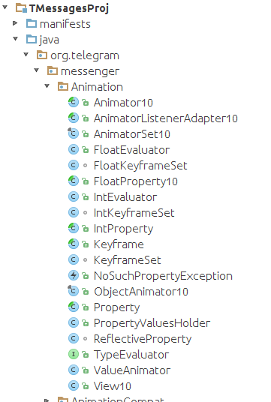
\includegraphics{imagens/telegram_diretorio.png}
\caption{Estrutura parcial dos pacotes do Telegram}
\label{fig:telegram_diretorio}
\end{figure}

Os resultados dos critérios de avaliação dessa técnica, apresentados na tabela 
\ref{tab:criterios_reimplementacao}, são semelhantes aos do pacote de
compatibilidade. Diferenciando em três critérios apenas: i) reusabilidade;
ii) legibilidade e; iii) tamanho da aplicação. A reusabilidade é alta em relação
à própria aplicação, mas baixa em relação a outras aplicações. Legibilidade é
prejudicada por aumentar a quantidade de pacotes e classes na aplicação. Esses
dois aspectos podem ser melhorados convertendo esse conjunto de classes em uma
projeto separado, sendo integrado a aplicação da mesma forma que pacotes de
compatibilidade. No entanto, como a reimplementação é feita apenas do que será
utilizado, o impacto no tamanho da aplicação é menor, em relação ao pacote de
compatibilidade.

\begin{table}[ht]
\centering
\caption{Descrição de reimplementação de recurso segundo o framework de comparação}
\label{fig:criterios_reimplementacao}
\begin{tabular}{|l|l|}
\hline
\multicolumn{1}{|c|}{\textbf{Critério de Avaliação}}                                                    & \multicolumn{1}{c|}{\textbf{Valor obtido}} \\ \hline
Tipo de Variabilidade                                                                                   & Positivo                                   \\ \hline
Variabilidade na estrutura                                                                              & Oferece suporte                            \\ \hline
Variabilidade no comportamento                                                                          & Oferece suporte                            \\ \hline
Granularidade                                                                                           & Grossa                                     \\ \hline
Tempo de ligação                                                                                        & Compilação                                 \\ \hline
Reusabilidade                                                                                           & Médio                                      \\ \hline
Legibilidade                                                                                            & Médio impacto                              \\ \hline
Desempenho                                                                                              & Baixo impacto                              \\ \hline
Tamanho da aplicação                                                                                    & Baixo impacto                              \\ \hline
\begin{tabular}[c]{@{}l@{}}Suporte para implementação\\ modular de requisitos transversais\end{tabular} & Não oferece suporte                        \\ \hline
\end{tabular}
\end{table}

A recomendação é evitar o uso de pacotes de compatibilidades quando o que será
utilizado é muito pouco \cite{multidex}. O que pode ser seguido por meio da
reimplementação do recurso desejado,
como feito pelo Telegram. Além
de evitar o aumento de métodos da aplicação que não serão utilizados, será possível
uma maior personalização do comportamento dos componentes, no entanto, é um elemento
a mais que os desenvolvedores deverão se preocupar em evoluir juntamente com o restante
da aplicação. Diferentemente dos pacotes de compatibilidade, cuja evolução é feita por
equipes dedicadas e externas ao projeto.

\subsubsection{Padrões de Projeto}
Foram ainda identificados alguns padrões de projeto para tratar variabilidades na API.

AnkiDroid e K-9 Mail aplicaram o padrão \textit{Strategy}. A primeira definiu uma
interface (\texttt{Compat}) com um conjunto de funções que não estão presentes em
todas as versões, e um conjunto de implementações dessa interface que irá prover
o suporte. Cada implementação deve terminar com um sufixo identificando a versão
mínima para essa implementação, ex. \texttt{CompatV12}. Existe uma implementação
\textit{default}, \texttt{CompatV10}, que provê suporte para API versão 10.
Nessa classe, os métodos da interface \texttt{Compat} relacionado à versão 10
da API realizam algum trabalho, enquanto os demais estão vazios, nada fazem ou
execução alguma ação secundária, como registrar (log) a chamada ou exibir alguma
informação para o usuário. As demais implementações
devem estender a implementação relacionado à versão anterior e implementar a
interface \texttt{Compat}. Cada implementação deverá sobrescrever somente os
métodos que surgiram na versão da classe. Métodos não suportados pela API
deverão manter a implementação padrão vazia.

O diagrama de classes parcial dessa
solução é apresentado na figura \ref{fig:strategy_uml}. Nesse diagrama, além
das classes já citadas, \texttt{CompatHelper} é uma classe auxiliar responsável,
entre outre coisas, por criar a estratégia concreta de acordo com a versão da API
do dispositivo, conforme mostra a figura \ref{fig:strategy}. \texttt{Cliente} representa um objeto qualquer
que necessite usar os serviços providos por uma das estratégias. Existem também outras
6 implementações concretas de \texttt{Compat}, genericamente representados no diagrama por
\texttt{CompatV\_N}.

\begin{figure}[ht]
\centering
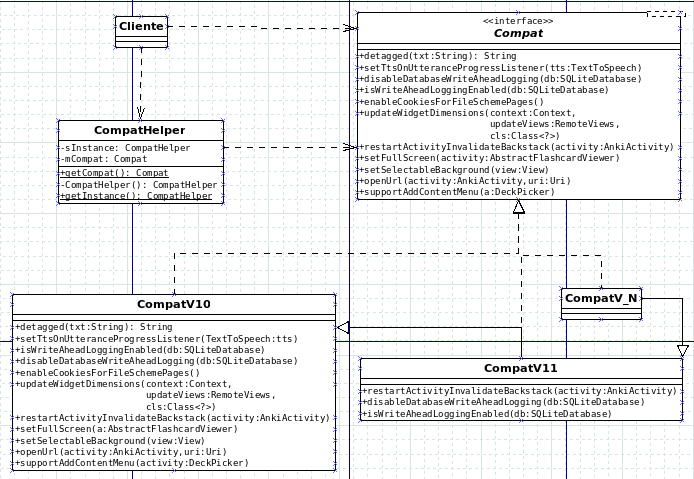
\includegraphics[width=1\textwidth]{imagens/strategy_uml.png}
\caption{Diagrama de classes parcial da solução adotada por AnkiDroid}
\label{fig:strategy_uml}
\end{figure}

\begin{figure}[ht]
\centering
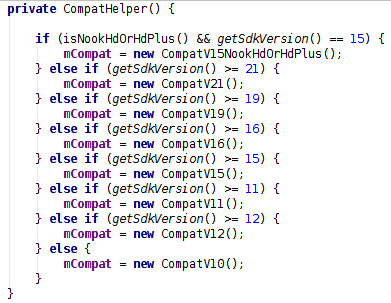
\includegraphics[width=0.5\textwidth]{imagens/strategy.png}
\caption{Criação de objetos concretos no padrão Strategy definida pela versão da API}
\label{fig:strategy}
\end{figure}

K-9 Mail especificou duas subclasses de \texttt{WebViewCompat}, uma que será instanciada com API’s inferiores a 21 e a outra para as demais.

Um aspecto chave no padrão \textit{Strategy} é a seleção do objeto concreto.
No exemplo apresentado, tal seleção ocorre em tempo de execução e no momento da
criação do objeto. Para uso dessa solução é necessário, de alguma forma, que a
aplicação seja capaz de pelo menos indicar o objeto a ser criado. Em alguns situações,
isso não é possível, impedindo o  tratamento da variabilidade na criação do objeto,
sendo necessário utilizar outra técnica. Na plataforma Android, isso geralmente
ocorre com elementos de interface gráfica, que herdam da classe \texttt{View} e
são instanciados pela própria plataforma.

Para essa situação, Telegram e c:geo utilizaram o padrão de projeto \texttt{Proxy}.
A figura \ref{fig:proxy_package_uml} apresenta um diagrama parcial de pacote e
classe da implementação do Telegram.

\begin{figure}[ht]
\centering
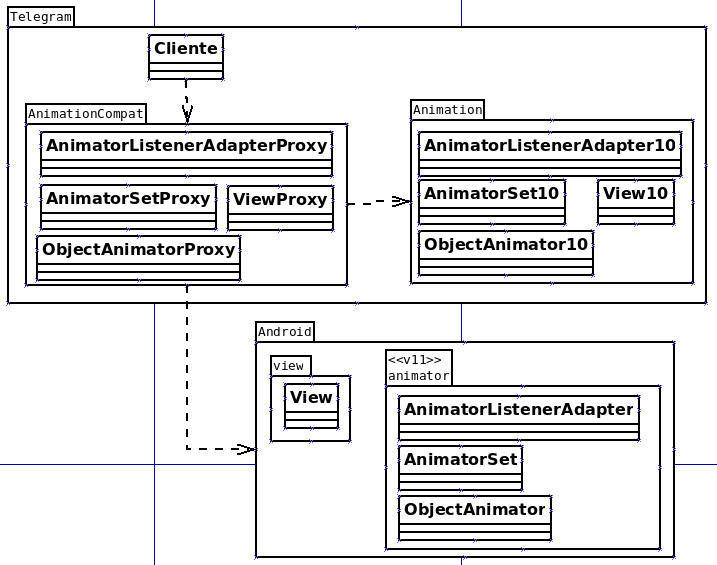
\includegraphics[width=0.75\textwidth]{imagens/proxy_package_uml.png}
\caption{Diagrama de pacote e classes do padrão Proxy no Telegram}
\label{fig:proxy_package_uml}
\end{figure}


Telegram definiu 4 classes \textit{proxies}, organizadas no pacote \texttt{AnimationCompat}.
Essas 4 classes são equivalente à classe \texttt{android.view.View}, que teve
métodos e comportamentos adicionados na versão 11 da biblioteca, e outras 3 classes
do pacote \texttt{android.animator}, que também só existe a partir da versão 11 da API.
O objetivo desse conjunto de classes é prover animações para objetos. Quando em
execução em um dispositivo com versão da API igual ou superior a 11, as classes
\textit{proxies} farão chamadas às classes do próprio sistema, caso contrário,
serão chamadas classes do pacote \texttt{animation}, do próprio Telegram. 

Tomando como exemplo objetos da classe \texttt{View}, a figura \ref{fig:exemplo_view_proxy}
apresenta uma sequencia de chamadas de métodos. Quando é necessário acessar um
método qualquer a classe cliente deverá acessar \texttt{ViewProxy} (1),  que
verificará a versão da API e fará a chamada adequada, seja para classe
\texttt{View10} ou para o próprio objeto alvo (2.a ou 2.b).


\begin{figure}[ht]
\centering
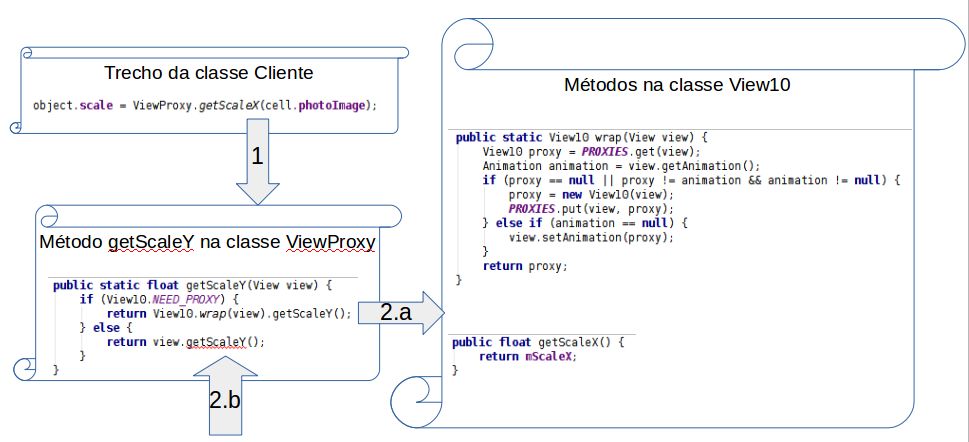
\includegraphics[width=1\textwidth]{imagens/exemplo_view_proxy.png}
\caption{Diagrama de pacote e classes do padrão Proxy no Telegram}
\label{fig:exemplo_view_proxy}
\end{figure}

Nessa aplicação do padrão \textit{Proxy}, existem duas importantes alterações em
relação ao seu uso mais comum:
\begin{itemize}
    \item A classe cliente é responsável por fornecer ao \textit{proxy} o objeto
        que será encapsulado (no exemplo, \texttt{cell.photoimage});
    \item Embora os \textit{proxies} possuam os mesmos métodos que o objeto real,
    eles não implementam a mesma interface Java, no sentido do uso da palavra-chave \texttt{extends}.
\end{itemize}

Esse solução também se fez necessário pelo fato do Telegram ter reimplementado os
recursos de animação, como foi detalhado na seção \ref{sec:reimplementacao},
e não estar usando pacotes de compatibilidade.

c:geo utilizou dois padrões de projeto: \textit{Null Object} e \textit{Decorator}.
Para o \textit{Null Object} foram definidos 3 elementos para cada versão da API
a qual se deseja oferecer suporte: (i) uma interface com os métodos; (ii) uma
classe que implementa essa interface e; (iii) uma outra que também implementa mas
os seus metodos nada fazem, é o “null object”.

Essa estrutura é encapsulada para as classes clientes em uma classe \texttt{Compatibility},
responsável por instanciar os objetos, receber a chamada do cliente e delegar para
o objeto. O diagrama de classe dessa solução é apresentado na figura \ref{fig:null_object}.

O padrão \textit{Decorator} é utilizado para permitir a alteração do tema de
\textit{activities} em versões da API anteriores a 11. Neste caso, a classe decoradora
\texttt{ContextThemeWrapper} é fornecida pela própria API. Nas versões superiores
ou igual a 11, essa modificação de tema já é disponível nativamente.
A figura \ref{fig:decorator} mostra uma adaptação desse código.
\begin{figure}[ht]
\centering
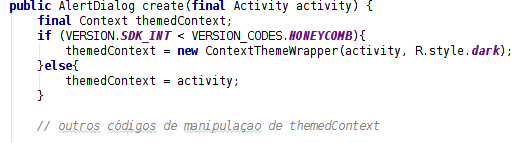
\includegraphics[width=1\textwidth]{imagens/decorator.png}
\caption{Utilização do padrão Decorator}
\label{fig:decorator}
\end{figure}


\begin{figure}[H]
\centering
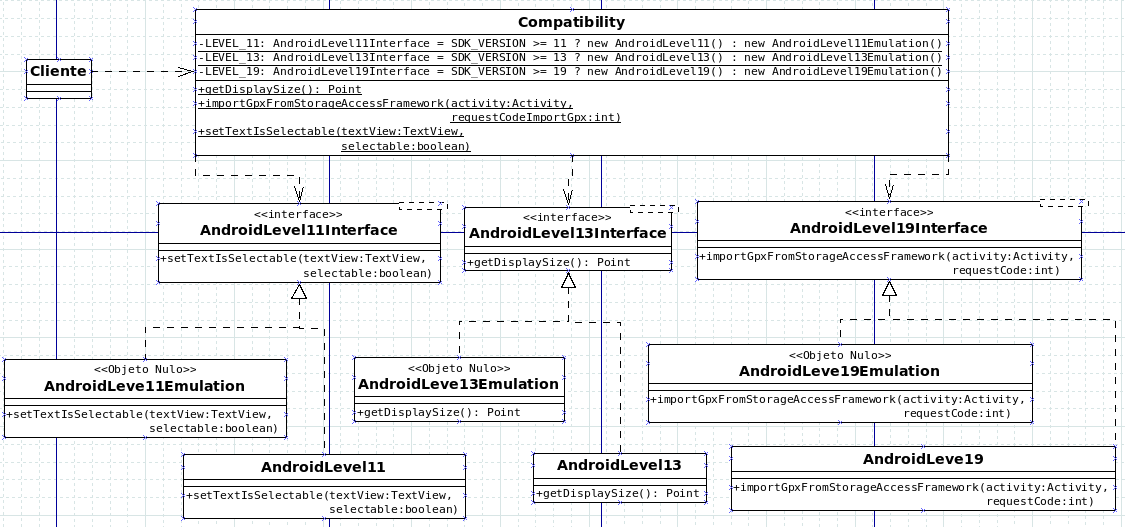
\includegraphics[scale=0.6, angle=90]{imagens/null_object.png}
\caption{Digrama de classes do padrão Null Object no c:geo}
\label{fig:null_object}
\end{figure}


A tabela \ref{tab:criterios_padroes} sintetiza os valores obtidos para os padrões
de projeto segundo o framework de comparação. 

\begin{table}[ht]
\centering
\caption{Síntese dos padrões de projeto segundo o framework de comparação}
\label{tab:criterios_padroes}
\begin{tabular}{|l|l|}
\hline
\multicolumn{1}{|c|}{\textbf{Critério de Avaliação}}                                                    & \multicolumn{1}{c|}{\textbf{Valor obtido}}                                                                                         \\ \hline
Tipo de Variabilidade                                                                                   & \begin{tabular}[c]{@{}l@{}}Positivo (Decorator),\\ Ambos(Strategy, Null Object, Proxy)\end{tabular}                                \\ \hline
Variabilidade na estrutura                                                                              & Oferece suporte (Decorator)                                                                                                        \\ \hline
Variabilidade no comportamento                                                                          & Oferece suportada (Decorator, Strategy, Null Object, Proxy)                                                                        \\ \hline
Granularidade                                                                                           & \begin{tabular}[c]{@{}l@{}}Grossa(Decorator, Strategy, Proxy),\\ Fina (Null Object)\end{tabular}                                   \\ \hline
Tempo de ligação                                                                                        & \begin{tabular}[c]{@{}l@{}}Execução (Decorator, Strategy, Null Object),\\ Compilação (Proxy)\end{tabular}                          \\ \hline
Reusabilidade                                                                                           & Alta (Decorator, Strategy, Null Object)                                                                                          \\ \hline
Legibilidade                                                                                            & \begin{tabular}[c]{@{}l@{}}Baixo impacto(Decorator, Strategy),\\ Médio impacto (Proxy),\\ Alto impacto (Null Object)\end{tabular} \\ \hline
Desempenho                                                                                              & \begin{tabular}[c]{@{}l@{}}Baixo impacto(Decorator, Strategy, Null Object),\\ Médio Impacto (Proxy)\end{tabular}                   \\ \hline
Tamanho da aplicação                                                                                    & \begin{tabular}[c]{@{}l@{}}Baixo impacto(Decorator),\\ Médio impacto (Strategy, Null Object, Proxy)\end{tabular}                   \\ \hline
\begin{tabular}[c]{@{}l@{}}Suporte para implementação\\ modular de requisitos transversais\end{tabular} & Não oferece suporte                                                                                                                \\ \hline
\end{tabular}
\end{table}

Como alguns padrões de projeto foram identificados, é necessário que a avaliação
seja feita separadamente. Cada padrão possui suas propriedades. O padrão \textit{Proxy}
utilizado levou a uma grande dispersão do código verificador da necessidade do \textit{proxy},
ocorrendo dentro de todos os métodos do próprio \textit{proxy}. Também houve um
detalhe importante na forma implementação entre as duas aplicações que o utilizaram:
no Telegram, essa implementação está no código da própria aplicação, enquanto no
c:geo em uma biblioteca de terceiros, estaticamente incorporada através do código
fonte. As demais aplicações não tiveram necessidade dessa solução porque ela é
usada para prover suporte às aplicações em execução sob a versão 9 da API.

A solução adotada pela aplicação AnkiDroid ao utilizar o padrão \textit{Strategy}
mostrou-se bastante efetiva, onde cada classe  que representa uma “estratégia concreta”
implementa especificamente os métodos que sofreram alteração entre as versões,
herdando os demais métodos das versões imediatamente anterior.
A aplicação K-9 Mail também utilizou \textit{Strategy}, mas não há relação de
herança entre as classes “estratégia” e elas são somente duas.

O padrão \textit{Strategy} também poderia ter sido utilizado na aplicação c:geo,
no entanto, foi escolhido o padrão \textit{Null Object}. Essa solução é de baixa
legibilidade, sendo necessária a implementação de 3 elementos para cada versão da
API a ser oferecido suporte: (i) uma interface com os métodos; (iii) uma classe
que implementa essa interface e; (iii) outra classe que também implementa essa interface
mas os seus metodos nada fazem, é o “null object”.
Além disso, como as interfaces são diferentes, não é possível usar polimorfismo,
e a programação é específica para cada implementação, demonstrando assim ser uma
solução dificil de manter. Atualmente, 3 versões foram suportadas: 11, 13 e 19.

Por fim, o padrão \textit{Decorator} utilizado pela aplicação c:geo foi beneficiado
pelo fato da classe decoradora ser da própria biblioteca padrão do Android,
sendo necesário apenas o acréscimo no código da verificação se será ou não
necessário fazer a decoração.

\subsection{Mudanças na API com Maior Impacto no Desenvolvimento}
\label{sec:mudancas}

A maioria das variações ocorridas ao longo da evolução da API e que sofreram algum
tipo de tratamento pelas aplicações analisadas dizem respeito à interface gráfica.
Tanto em relação a animações \texttt{pacote android.animator} durante alguma ação
quanto para utilizar a API de fragmentos, que foram adicionados ao Android apenas
na versão 11. Para esses casos, o mais comum é o uso do pacote de compatibilidade.

O pacote \texttt{android.animator} foi o recurso implementado pelo Telegram citado
na seção \ref{sec:reimplementacao}. Além disso, um dos elementos utilizados por
Telegram e somente por ele foi a \textit{tag} XML (EXtensible Markup Language) \texttt<vector>,
disponibilizada
na versão 21 e que permite a definição de uma imagem vetorial, que será renderizada
em tempo de execução pela plataforma em adequação às dimensões da tela. O uso desse
recurso, simplifica o desenvolvimento, já que não será necessário criar diversas
imagens repetidas em função das diferentes telas, e na diminuição do tamanho dos
arquivos APKs, já que essas imagens serão criadas em tempo de execução.

Firefox utilizou dois pacotes que só foram adicionados em versões da plataforma
superiores a versão mínima do aplicativo: \texttt{android.hardware.input} e
\texttt{android.print}. Firefox é também a aplicação que mais utiliza recursos
de versões posteriores à mínima necessária, apesar de, juntamente com K-9 Mail,
possuir a maior versão mínima (15) dentre as aplicações analisadas.

O elemento mais utilizado por aplicações é uma tag XML para definição da família
da fonte de objetos da classe \texttt{TextView}: \texttt{<android:fontFamily>}.
Ela ocorreu em 3 aplicações. Um outro que ocorreu em mais de uma aplicação é o
método \texttt{android.app.AlarmManager \#setExact} que foi adicionado na versão
19 para tratar um comportamento do sistema de relógio do Android que sofreu
alterações nessa versão. É utilizado por Firefox e Zmanim, este último muito
dependente do relógio do dispositivo.

Foi identificada uma grande granularidade de recursos tratados entre as aplicações,
ou seja, muitas classes e métodos por aplicação e pouca repetição de uma aplicação
para outra.
 
Dois motivos podem ter contribuído para isso:
\begin{itemize}
    \item A versão mínima das aplicações: metade das aplicações analisadas possuem
        versao mínima superior a 11, quando foi introduzida a API de fragmentos e
        vários outros novos recursos comuns. Além disso, elementos dos pacotes
        de compatibilidade não foram identificados nessa análise;
   \item Uso da regra Lint NewAPI para análise: ao usar essa regra, elementos
        mais recentes e comuns, mas ainda assim inferiores a versão mínima da
        aplicação não foram identificados. Por exemplo, a API de fragmentos em
        aplicações com versão mínima igual ou superior a 11.
\end{itemize}


Para uma análise mais precisa é necessário considerar as alterações da API
utilizada pelas aplicações e que sejam anteriores a sua versão mínima e os
elementos do pacote de compatibilidade utilizados. Outro possível fator dessa
diversidade é a variedade de categorias das aplicações analisadas. Foram 8
aplicações de 6 categorias.

\subsection{Tratamento de Múltiplas Telas}
\label{sec:multiplas_telas}

Para oferecer um suporte adequados para diferentes dispositivos, as aplicações
devem: (i) desenhar layouts otimizando o espaço disponível; e (ii) disponibilizar
imagens de tamanhos diferentes, de forma que não necessitam ser redimensionadas
pela plataforma em tempo de execução.

Das aplicações analisadas, duas delas - c:geo e Zmanim - estão disponíveis apenas
para celulares, sendo desnecessários \textit{layouts} otimizados e outras duas - Firefox
e K-9 Mail - não possuem tal recurso. No entanto, apenas Zmanim não disponibilizou
imagens de tamanhos diversos.

Embora o arquivo contendo a descrição do \textit{layout} seja carregada pela própria
plataforma, sendo transparente para a aplicação, em algumas situações pode ser
necessário a verificação explícita do tipo de dispositivo, em especial para
distinguir entre celular e \textit{tablet}. Essa verificação foi detectada no Firefox
e no Telegram.

Foi possível executar quatro aplicações em dois aparelhos reais diferentes,
um celular de tela pequena com versão 2.3.4 do Android (API 10) e um \textit{tablet} com
versão Android 4.1.1 (API 16). Em duas aplicações - AnkiDroid e Telegram  - foi perceptível
o layout diferente em função dos espaços disponíveis. AntennaPod e K-9 Mail possuem
o mesmo layout em ambos aparelhos. Não foi possível fazer essa análise com mais
aplicações porque ou não eram compativeis com o tipo de aparelho, ou com a versão
do Android. Tal tipo de restrição oferecida pela plataforma, ajuda a evitar
interrupções no uso da aplicação, no caso de versões da API, ou que o usuário
tenha uma experiência de uso não desejada para o caso dos dispositivos.

A tabela \ref{tab:multiplos_pacotes} resume o descrito acima.

\begin{table}[ht]
\centering
\caption{Resumos do tratamento das aplicações em relação a telas de tamanhos diferentes}
\label{tab:multiplos_pacotes}
\begin{tabular}{|l|c|c|c|c|}
\hline
\textbf{Aplicação} & \textbf{\begin{tabular}[c]{@{}c@{}}Aparelhos\\ Alvo\end{tabular}} & \textbf{\begin{tabular}[c]{@{}c@{}}Layouts\\ Especializados\end{tabular}} & \textbf{\begin{tabular}[c]{@{}c@{}}Imagens\\ Especializadas\end{tabular}} & \textbf{\begin{tabular}[c]{@{}c@{}}Verificação\\ Explicita\end{tabular}} \\ \hline
AnkiDroid          & Ambos                                                             & X                                                                         & X                                                                         &                                                                          \\ \hline
AntennaPod         & Ambos                                                             &                                                                           & X                                                                         &                                                                          \\ \hline
c:geo              & Celular                                                           & Não aplicável                                                             & X                                                                         & Não aplicável                                                            \\ \hline
Firefox            & Ambos                                                             &                                                                           & X                                                                         & X                                                                        \\ \hline
Google I/O         & Ambos                                                             & X                                                                         & X                                                                         &                                                                          \\ \hline
K-9 Mail           & Ambos                                                             &                                                                           & X                                                                         &                                                                          \\ \hline
Telegram           & Ambos                                                             & X                                                                         & X                                                                         & X                                                                        \\ \hline
Zmamin             & Celular                                                           & Não aplicável                                                             &                                                                           & Não Aplicável                                                            \\ \hline
\end{tabular}
\end{table}

Duas aplicações, c:geo e Zmanim, sempre serão instaladas em dispositivos de telas
com tamanhos bem parecidos, portanto, não há tratamento em relação a esse quesito.
Para a aplicação c:geo isso é da natureza de  aplicações de \textit{geocaching} \cite{Ohara2008},
que pressupõe uma maior mobilidade. O que não acontece com a aplicação Zmanim,
que poderia ser beneficiada com uma maior base de usuários caso fosse possível
a instalação em \textit{tablets}.

Três aplicações - AnkiDroid, AntennaPod e Google I/O -  compõem o \textit{layout}
da aplicação por meio do arranjo de fragmentos. No entanto, apenas em AnkiDroid
e Google I/O esse arranjo é baseado no tamanho da tela. Em AntennaPod, os
fragmentos são apenas subsituídos quando o usuário acessa funções diferentes do
aplicativo, não se beneficiando de telas maiores.

Firefox e K-9 Mail não utilizam fragmentos. No Firefox isso pode ser explicado
também pelo objetivo da aplicação. Um navegador contém apenas uma região de
conteúdo ocupando toda a tela é o comportamento padrão e já esperando pelos
usuários. A aplicação K-9 Mail, assim como AntennaPod, poderia se beneficiar de
telas de tamanhos diferentes e propiciar uma melhor experiência para seus usuários.

\subsection{Múltiplos Pacotes para Instalação}
\label{sec:multiplos_pacotes}

Embora seja possível um único pacote de instalação prover suporte para diversos
dispositivos, e esse seja o recomendado \cite{multiple_apks}, a Play Store
permite que os distribuidores das aplicações enviem pacote customizados e especializados.

Quando o usuário faz uma busca diretamente do aparelho, a Play Store identifica as
configurações do dispositivo e disponibiliza para instalação o pacote apropriado.
As configurações atualmente possíveis para customização dos APKs são:
\begin{itemize}
    \item diferentes formatos de compressão para textura OpenGL;
    \item diferentes tamanhos e densidades de telas;
    \item diferentes recursos de hardware dos aparelhos;
    \item diferentes versões da plataforma;
    \item diferentes arquiteturas da CPU (ARM, x86 e MIPS, entre outras)
\end{itemize}

Somente 4 aplicações disponibilizam múltiplos pacotes para instalação: AntennaPod,
Firefox, K-9 Mail e Telegram. No entanto, analisando o código fonte e o processo
de compilação de tais aplicações não foram encontradas estruturas que levassem 
criação de diferentes pacotes. Possivelmente, os desenvolvedores optaram por
atualizar a versão mínima da plataforma, evitando ter que manter compatibilidade
com dispositivos mais antigos, mas deixaram esses pacotes como forma de ainda
atender tais dispositivos.

Um possível fator para o baixo uso de múltiplos pacotes é sua complexidade de
desenvolvimento e publicação, sendo preferível um único pacote que ofereça suporte
para todos os dispositivos. Uso de múltiplos pacotes é indicado quando um único
APK fica maior que 100MB.

\subsection{Ferramentas Úteis para Tratar Variabilidades}
\label{sec:ferramentas}

Algumas ferramentas oficiais, integradas ao Android Studio, podem ser bastante úteis
para gerencia de variabilidades.

\subsubsection{Android Library}
Android Library é um projeto Android que possui a mesma estrutura de uma aplicação,
incluindo código-fonte, arquivos de recursos, e um arquivo manifesto. No entanto,
é compilado para um Android Archive (AAR) e não um Android Package (APK),
e que será utilizado como uma dependência para uma aplicação Android.

Isto é útil quando se deseja:
\begin{itemize}
    \item construir diversas aplicações que usem alguns dos mesmos componentes,
        como atividades, serviços ou layouts;
    \item construir aplicações que serão distribuídas em múltiplas APK com
        funcionalidade diferentes mais que utilizam os mesmos componentes básicos.
\end{itemize}

\subsubsection{Build Variant}
\textit{Build Variant} é um recurso do sistema de construção de aplicações Android
que permite a criação de diferentes versões de uma mesma aplicação. Existe dois
tipos motivos principais para uso desse recurso:
\begin{enumerate}
    \item Diferentes versões da mesma aplicação. Por exemplo, uma versão paga e
        outra gratuita.
    \item Mesma aplicação distribuída em múltiplos APK no Play Store.
    \item Uma combinação de 1 e 2.
\end{enumerate}

Cada build variant é composto de dois elementos: \textit{product flavor} e
\textit{build type}. Enquanto \textit{build type} está associado a configurações
de compilação e empacotamento e opções de depuração, um \textit{product flavor}
define uma versão customizada da aplicação. Um único projeto pode conter
diferentes \textit{product flavors}.

Tipicamente, são definidos dois \textit{build types} por projetos (\textit{debug}
e \textit{release}) e
considerando uma aplicação com 2 \textit{product flavor} (Flavor1 e Flavor2),
4 \textit{build variants} seriam criadas:
\begin{enumerate}
    \item Flavor1 - debug
    \item Flavor1 - release
    \item Flavor2 - debug
    \item Flavor2 - release
\end{enumerate}

O objetivo primário do \textit{build variant} é a criação de diferentes APKs
para o mesmo projeto, em oposição a dois projetos compartilhando a mesma Android Library.

\subsubsection{Análise do uso pelas aplicações}
A tabela \ref{tab:uso_ferramentas} indica quais ferramentas são utilizadas pelas
aplicações analisadas. Para Android Library, foi considerado a existência de qualquer
módulo do projeto configurado como library. Para Build Variant, foi verificada a
existência da opção \texttt{productFlavors} no arquivo \texttt{build.gradle} da
aplicação configurado com algum \textit{product flavor} definido.

\begin{table}[ht]
\centering
\caption{Uso das ferramentas por aplicação}
\label{tab:uso_ferramentas}
\begin{tabular}{|l|c|c|}
\hline
\textbf{Aplicação} & \textbf{Android Library} & \textbf{Build Variant} \\ \hline
AnkiDroid          & X                        &                        \\ \hline
AntennaPod         & X                        &                        \\ \hline
c:geo              & X                        & X                      \\ \hline
Firefox            &                          & X                      \\ \hline
Google I/O         &                          &                        \\ \hline
K-9 Mail           & X                        &                        \\ \hline
Telegram           &                          &                        \\ \hline
Zmamin             &                          & X                      \\ \hline
\end{tabular}
\end{table}

O conceito por trás de Android Library, uso de bibliotecas de código, é comum na
engenharia de software. Encontramos módulos do tipo Android Library em 4 aplicações:
AnkiDroid, AntennaPod, c:geo e K-9 Mail.
A aplicação Zmanim não utiliza esse tipo de módulo mas utiliza outras bibliotecas
Java de propósito mais geral, não específica para Android.

Build Variant é uma tecnologia relativamente nova, e para estruturar uma aplicação
com esse recurso é necessário experiencia do engenheiro de software. Motivos pelo
qual apenas 3 aplicações utilizam tal recurso: c:geo, Firefox e Zmanim.
Ainda assim, Firefox utiliza apenas
para se beneficiar de um recurso existente na versão 21 do Android que permite
uma compilação mais rápida. Além disso, como foram avaliadas apenas aplicações
\textit{open-source} e gratuitas, não faz sentidos versões “demo” e “premium”,
o que justificaria um maior uso de \textit{build variants}.


